\documentclass[fleqn]{article}
\usepackage[utf8]{inputenc}
\usepackage{geometry}
\usepackage{fancyhdr}
\usepackage{amsmath,amsthm,amssymb}
\usepackage{graphicx}
\usepackage{hyperref}
\usepackage{lipsum}
\usepackage{ulem}
\usepackage{comment}
\usepackage{enumerate}
\usepackage{titlesec}

% custom commands
\newcommand{\leadingzero}[1]{\ifnum #1<10 0#1\else#1\fi}
\newcommand{\gerdate}[3]{\leadingzero{#1}.\leadingzero{#2}.\leadingzero{#3}}
\newcommand{\gertoday}{\gerdate{\the\day}{\the\month}{\the\year}}
\newcommand*{\bfrac}[2]{\genfrac{}{}{0pt}{}{#1}{#2}}
\newcommand{\R}{\mathbb{R}}
\newcommand{\N}{\mathbb{N}}
\newcommand{\Q}{\mathbb{Q}}

\setcounter{section}{0}
\setcounter{subsection}{0}
\pagestyle{fancy}

\lhead{Tom Vogt, Tobias Knöppler}
\chead{}
\rhead{\gertoday}
\lfoot{}
\cfoot{\thepage}
\rfoot{}
\setlength{\mathindent}{0pt}

% document specific settings
\renewcommand{\thesection}{}
\renewcommand{\thesubsection}{\arabic{section}. \alph{subsection})}
\renewcommand{\thesubsubsection}{\roman{subsubsection})}
\titleformat{\subsubsection}[runin]{\normalfont\normalsize\bfseries}{\thesubsubsection}{1em}{}

\title{Diskrete Mathematik - Hausaufgaben zum 5. Dezember 2014 (Blatt 07)}
\author{Tobias Knöppler (Matr-Nr: 6523815), Thomas Vogt (Matr-Nr.: 6687486)}
\date{\gertoday}
\begin{document}
\maketitle

\section{}

\subsection{}%subsection name}\label{label}
Da eine Kante je zwei Knoten verbindet, erhöht sie auch den Grad von zwei Knoten. Damit lässt sich die Anzahl der Kanten wie folgt ermitteln, wobei $g_i$ den Grad des i-ten Knoten bezeichnet.
$\frac{\sum\limits_{i=1}^{100} g_i}{2} = \frac{50 \cdot 3 + 30 \cdot 4 + 20 \cdot 6}{2} = \frac{390}{2} = 195$\\
Der Graph hat also 195 Kanten.

\subsection{}%subsection name}\label{label}

\textbf{Anmerkung: } Ich gehe hierbei von einem ungerichteten Graphen aus, da dies in der Aufgabenstellung nicht weiter angegeben wurde.
\begin{itemize}
    \item[I] Die Knotenmenge enthält 5 Elemente. Damit kann man $\left(\bfrac{2+5-1}{2}\right) = \frac{(6)^{\underline{2}}}{2!} = \frac{6 \cdot 5}{2} = 15$ verschiedene ungeordnete Tupel aus der Menge bilden (Die Menge der Tupel bezeichne ich im folgenden als T). Diese stellen die möglichen Kanten im Graphen dar.
    \item[II] Alle möglichen Kombinationen dieser Tupel entsprechen damit allen möglichen Graphen, welche aus der Knotenmenge \{1, 2, 3, 4, 5\} gebildet werden könne; diese werden durch die Potenzmenge $P(T)$ beschrieben.
    \item[III] Damit gibt es $P(T) = 2^{|T|} = 2^{15}$ verschiedene Graphen, die aus der Knotenmenge \{1, 2, 3, 4, 5\} gebildet werden können.
\end{itemize}

\section{}%section name}\label{label}
\subsection{}%subsection name}\label{label}
\begin{flalign*}
    A_1 &= \{1, 2, 3\}\\
    A_2 &= \{1, 2, 4\}\\
    f :&= \{\{1,a\}, \{2,b\}, \{3,c\}, \{4,c\}\}\\
    \Rightarrow f[A_1 \cap A_2] &= f[\{1, 2\}] = \{a,b\}\\
    \Rightarrow f[A_1] \cap f[A_2] &= \{a, b, c\} \cap \{a, b, c\} = \{a, b, c\}
\end{flalign*}

\subsection{}%subsection name}\label{label}
\begin{flalign*}
    B &= \{a, b\}\\
    B_1 &= \{a\}\\
    f :&= \{\{1, a\}, \{2, b\}, \{3, a\}\}\\
    f[f^{-1}[B_1]] = f[f^{-1}[a]] = f[{1, 3}] = {a}
\end{flalign*}

\section{}%section name}\label{label}

 Nein, da es z.B. im ersten Graph keine Kante zwischen zwei Knoten mit Grad 4 gibt, im zweiten jedoch schon.

\section{}%section name}\label{label}
Die Graphen 2 und drei sind isomorph. Ihre Strukturgleichheit lässt sich leicht einsehen, wenn man die die drei miteinander verbundenen Knoten im Innern des großen Rings nach außen bewegt; siehe Zeichnung:
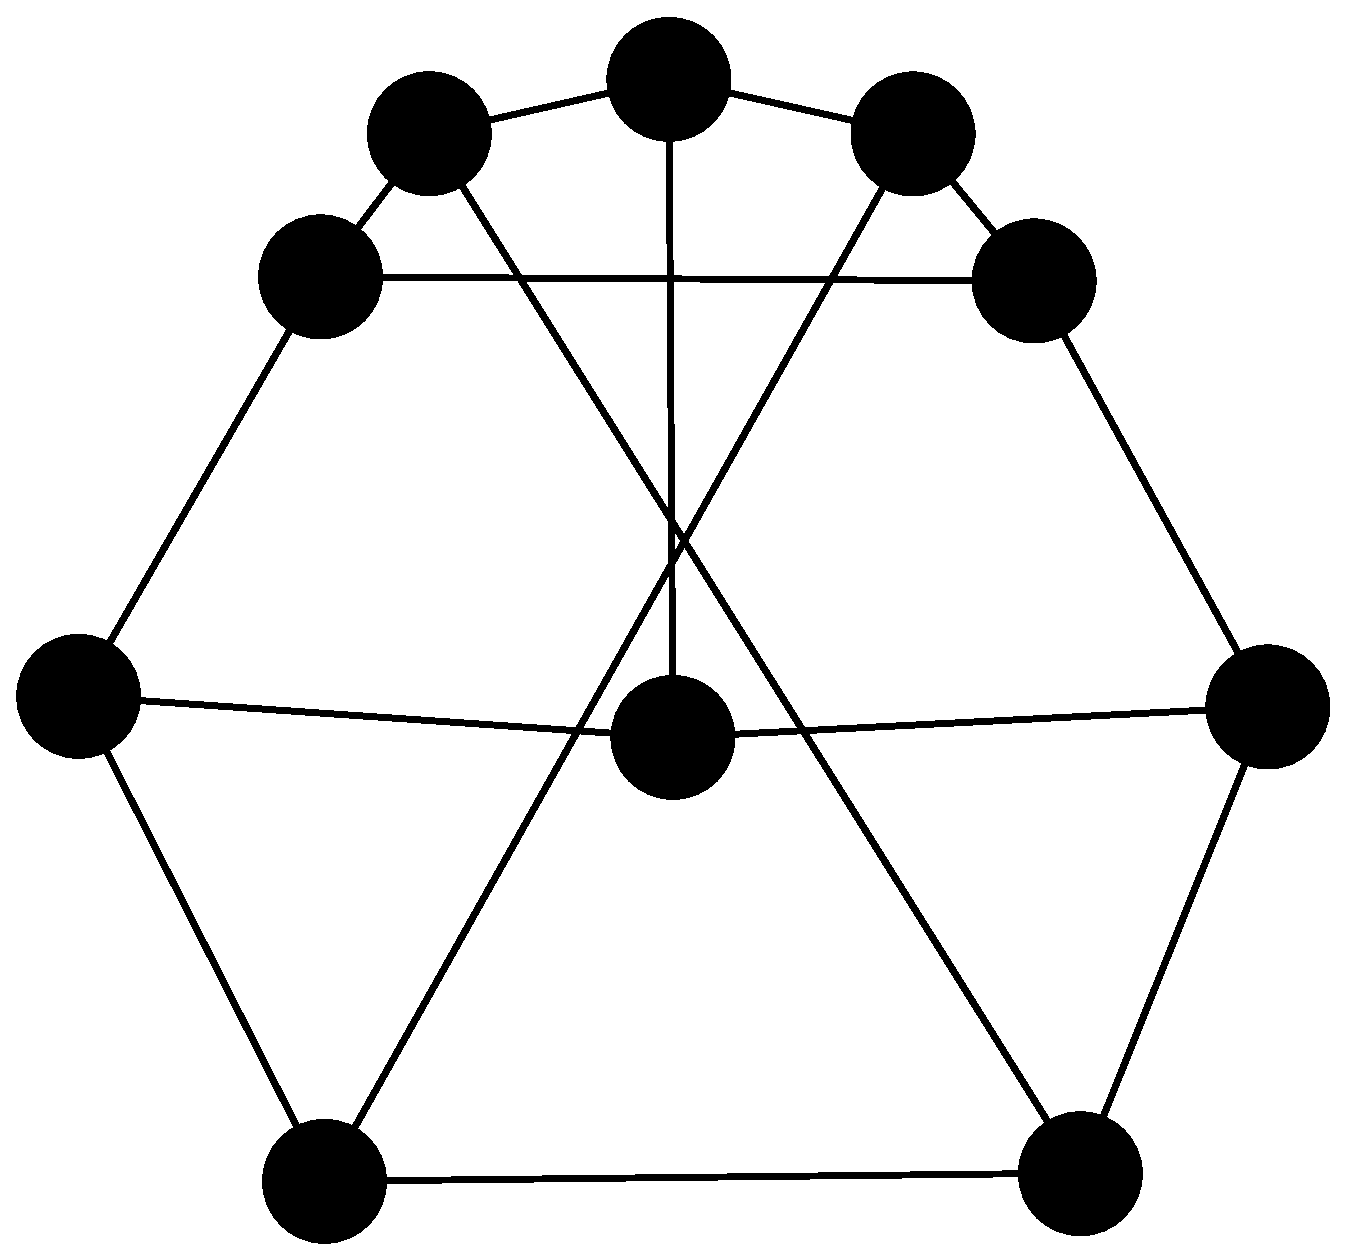
\includegraphics[scale=0.3]{iso2.eps}
Der erste Graph kann mit dem dritten Graphen nicht isomorph sein, da es keinen Ring in ihm gibt, der genau 10 Knoten enthielte. Da die anderen beiden Graphen isomorph sind, ist der erste Graph damit auch nicht mit dem zweiten Graphen isomorph.

\section{}%section name}\label{label}
\subsection{}%subsection name}\label{label}
Er hat $\left(\bfrac{10}{2}\right) = \frac{10 \cdot 9}{2} = 45$ Kanten.
\subsection{}%subsection name}\label{label}
Da jedes Element in einem vollständigen Graphen eine Kante zu jedem anderen Element besitzt, entspricht dieses Problem der Frage, wie viele Möglichkeiten es gibt, 3 Elemente aus einer 10-elementigen Teilmenge zu ziehen, wobei die Reihenfolge unwichtig ist und die Elemente nach dem Ziehen jeweils wieder zurückgelegt werden.\\
Damit gibt es $\left(\bfrac{3 + 10 - 1}{3}\right) = \frac{12  \cdot 11 \cdot 10}{3 \cdot 2} = 220$ Kreise der Länge 3 in G.






\end{document}
